\chapter{Games}
Aún no ha pasado suficiente tiempo como para que se haya empleado Vulkan con una gran variedad de juegos. Pero ya
existen compañías que han empleado este motor para realizar desarrollos.

El primero en lanzar un juego con soporte de esta API ha sido \emph{Ashes of Singularity}, un juego de estrategia en
tiempo real. También fue el primer juego en dar soporte total a DirectX 12. En este casi ha resultado extraño que solo
han puesto a la venta el juego en Windows pudiendo haberlo sacado para el resto de plataformas.

\emph{Doom}, es uno de los primeros juegos en categoría AAA que  ofreció dar soporte a Vulkan a los pocos meses de ser
sacado a la venta. Típicamente \emph{ID Software}, la compañía que ha desarrollado la saga, ha trabajado desarrollando
sus juegos con la API de OpenGL. En este caso no ha sido diferente, aunque como extra han ofrecido la opción de usar
Vulkan con excelentes resultados.

Por parte de Valve, ha permitido implementar Vulkan en su motor Source 2. Juegos como \emph{Dota 2} han sido de los
primeros en implementar esta API, siendo de los primeros en dar soporte multiplataforma. \emph{Ark: Survival Evolver}
es otro título que ofrece un soporte plataforma con una muy buena calidad de juego.

Otros ejemplos de videojuegos que emplean Vulkan, tanto en escritorio como en dispositivos móviles, son
\emph{Vainglory}\ref{fig:vainglory}, \emph{Rust}, \emph{Need for Speed: No Limits}...

\begin{figure}[t]
	\begin{center}
		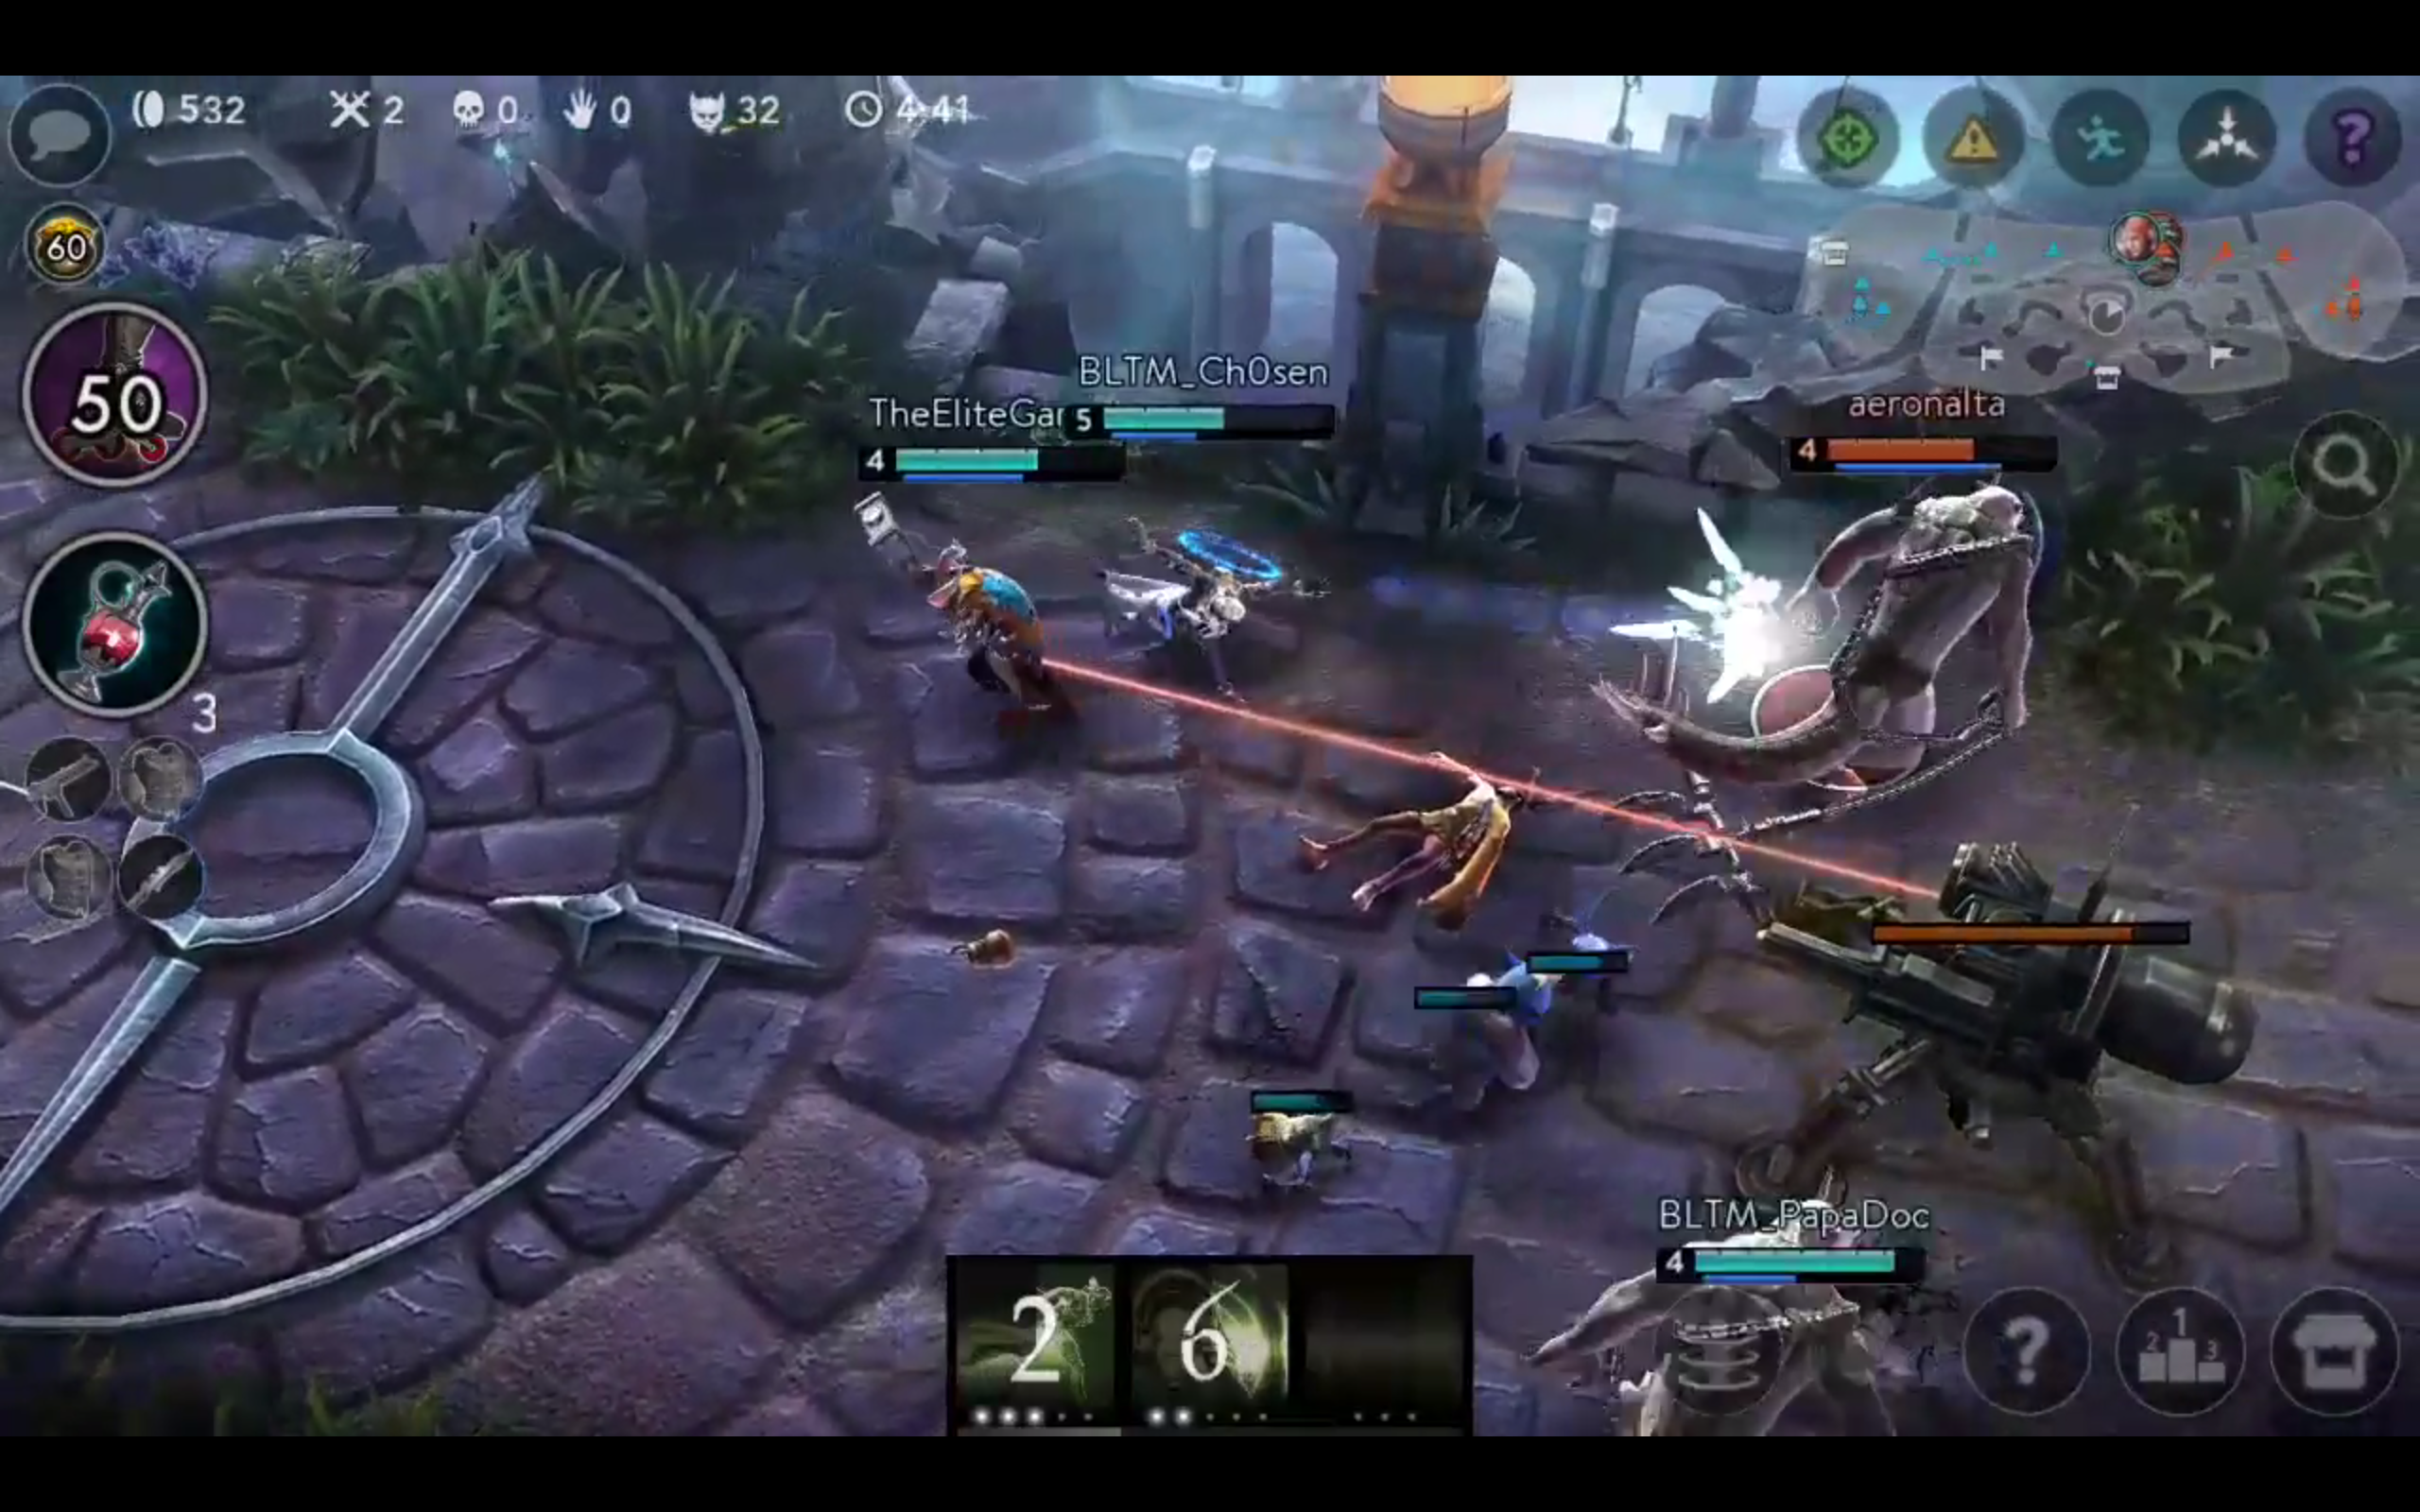
\includegraphics[scale=0.2]{galaxy_s7_edge-vainglory}
		\caption{\emph{Vainglory} ejecutado en un Samsung Galaxy S7 Edge}
		\label{fig:vainglory}
	\end{center}
\end{figure}
